\begin{center}
{\it by Diego Redigolo}
\end{center}

%\subsubsection{The singlet Higgs and the lifetime frontier at HL-LHC}
The existence of additional Higgs bosons is motivated by many
approaches to physics beyond the Standard Model. Here we focus on the simple case of a second Higgs which is a singlet of the SM gauge group. This is motivated in many BSM constructions addressing the naturalness problem of the electroweak scale like Supersymmetry or Compositeness. Independently on naturalness, an extra singlet arises in minimal scenarios to get a first-order EW phase transition which is necessary for EW baryogenesis. 

There is now an extensive suite of LHC searches for additional Higgs bosons decaying promptly into SM
final states. Among these, di-boson searches are particularly promising to hunt for an additional Higgs singlets (see Refs.~\cite{Sirunyan:2018qlb,Aaboud:2018knk,Sirunyan:2017isc,ATLAS:2017spa}). A first important question for HL-LHC is to understand how these direct searches correlate with Higgs coupling deviations. This question has already been addressed for the singlet Higgs at HL-LHC in Ref.~\cite{Buttazzo:2015bka} (see also Sec.~6.1.4 in the WG3 physics report \cite{CidVidal:2018eel} and Sec.~\ref{sec6:singletHP} of this report) and we summarise it here for completeness. In short, one can prove that there is limited room for discovery of the second Higgs singlet in direct production unless deviations in the SM Higgs coupling bigger than $5\%$ will be found at HL-LHC. This is a great motivation for future machines exploring the high energy frontier in SM visible decays of the second Higgs (see for example Ref.~\cite{Buttazzo:2018qqp} for an assessment of the reach of high-energy lepton colliders). 

Here we show that the situation is radically different if the second Higgs singlet has exotic displaced decays following Ref.~\cite{Alipour-fard:2018mre}. We focus on the case of a singlet Higgs decaying into a pair of long-lived particles (LLPs), whose decays within the detector volume set them qualitatively apart from promptly-decaying or detector-stable
particles. These type of displaced decays are often present in extensions of the Higgs sector which entail rich hidden sectors coupled primarily through the Higgs portal to additional Higgs-like scalars (see Ref.~\cite{Curtin:2018mvb} for a recent summary of the theory motivations).  

On the experimental side, the signatures of displaced LLP's pairs produced from the decay of a heavy singlet Higgs are sufficiently distinctive that they may be identified by analyses with little or no Standard Model backgrounds even at HL-LHC, making them a promising channel for discovering additional Higgs bosons. By recasting present LHC searches for a pair of displaced tracks with different displacements \cite{Aad:2015uaa,CMS:2014wda,Aaboud:2018aqj,Sirunyan:2018pwn}, we show that the discovery potential of exotic decays of the second Higgs singlet exceeds the asymptotic reach of SM Higgs coupling deviations and provides a natural avenue for the further development of searches for additional Higgs bosons. This is a promising next step to complete the experimental coverage of extended Higgs sectors at the LHC, especially because analogous decays of the 125 \UGeV Higgs to LLPs may be challenging to discover at the LHC due to trigger thresholds (see Ref.~\cite{Curtin:2013fra} for a summary and Refs.~\cite{Clarke:2015ala,Csaki:2015fba,Curtin:2015fna,Pierce:2017taw} for collider studies of displaced signal from SM Higgs decays).
  
On the theory side many models addressing dark matter, baryogenesis and the hierarchy problem can be mapped to the singlet simplified model we discuss here as long as the interactions of the heavy Higgs are controlled primarily by the Higgs portal. As an example, we present the concrete case of the Twin Higgs (TH) construction, quantifying the asymptotic reach of LHC searches for a Twin Higgs decaying into a pure glue hidden valley as originally proposed in Ref.~\cite{Craig:2015pha}. 

Regarding the physics opportunities of HE-LHC, we refer to \cite{CidVidal:2018eel} for a discussion of the visible decays of the singlet Higgs. A reliable assessment of the reach in exotic displaced decays strongly depends on the details of the trigger opportunities of HE-LHC and it is left for the future.    

\subsubsection{The simplified model with a long lived singlet scalar}

We introduce the effective Lagrangian of a CP-even scalar up to dimension four:
\begin{equation}
\mathcal{L}_{\text{visible}}=\frac{1}{2}(\partial_\mu S)-\frac{1}{2} m_S^2 S^2-a_{HS} S\vert H\vert^2-\frac{\lambda_{HS}}{2} S^2\vert H\vert^2-\frac{a_S}{3} S^3-\frac{\lambda_S}{4} S^4\ .\label{eq:everybody}
\end{equation}
After electroweak symmetry breaking, the singlet mixes with the uneaten CP-even component of the Higgs doublet and we can write the mixing angle $\gamma$ as
\begin{equation}
\gamma\simeq\frac{v(a_{HS}+\lambda_{HS} f)}{m_\phi^2}\quad\ ,\qquad H=\begin{pmatrix}\pi^+\\ \frac{v+h}{\sqrt{2}}\end{pmatrix}\quad\ ,\qquad S=f+\phi\ ,
\end{equation}   
where $m_\phi$ is the mass of the singlet in the mass basis, $v=246\text{ \UGeV}$ is the electroweak vacuum expectation value and $f$ is the VEV of the singlet $S$. The formula shows how the mixing between the singlet and the SM Higgs is controlled by the spontaneous and/or explicit breaking of a discrete $\mathbb{Z}_2$ symmetry under which the singlet is odd ($S\to -S$) and the SM Higgs even $(H\to H)$.  In what follows, we focus mainly on the scenario where the singlet takes a VEV at the minimum of a $\mathbb{Z}_2$-invariant potential. Then the $\mathbb{Z}_2$-breaking is spontaneous and we have
\begin{equation}
\gamma\simeq \frac{\lambda_{HS}}{\lambda_S}\cdot\frac{v}{f}\qquad ,\qquad m_\phi^2\simeq \lambda_S f^2\ . \label{eq:mixing}
\end{equation} 
 This is explicitly realised in Twin Higgs scenarios where $\lambda_S\simeq \lambda_{HS}$ and $\gamma\sim \frac{v}{f}$ (see Refs~\cite{Chacko:2005pe,Barbieri:2005ri}). The phenomenology of the singlet and the SM-like Higgs can be summarised as follows:
\begin{align}
&\frac{g_{hVV,f\bar f}}{g_{hVV,f\bar f}^{SM}}=\cos^2\gamma \label{eq:SMHiggs}\ ,\\
&\sigma_\phi=\sin^2\gamma\cdot \sigma_{h}(m_\phi)\label{eq:Sproduction}\ ,\\
&\text{BR}_{\phi\to f\bar{f},VV}=\text{BR}_{h\to f\bar{f},VV}(1-\text{BR}_{\phi\to hh\ \label{eq:SBR}
})\ ,
\end{align}
where $g_{hVV}/g_{hVV}^{SM}$ and $g_{hf\bar f}/g_{hf\bar f}^{SM}$ refer to the couplings of the SM-like Higgs to SM vectors and fermions, respectively, normalised to the SM prediction. The couplings of the SM-like Higgs in Eq. (\ref{eq:SMHiggs}) are reduced by an overall factor, leading to a reduced production cross section in every channel but unchanged branching ratios. The production cross section of the heavy singlet $\sigma_\phi$ in Eq. (\ref{eq:Sproduction}) is the one of the SM Higgs boson at mass $m_\phi$ rescaled by the mixing angle.  The branching ratios of the singlet into SM gauge bosons in Eq.~\eqref{eq:SBR} are rescaled by a common factor depending on the branching ratio into $hh$. The latter is model dependent but in the limit $m_\phi\gg m_W$ an approximate $SO(4)$ symmetry dictates $\text{BR}_{\phi\to hh }\simeq \text{BR}_{\phi\to ZZ}\simeq \text{BR}_{\phi\to WW} /2$.

\begin{figure}[t]
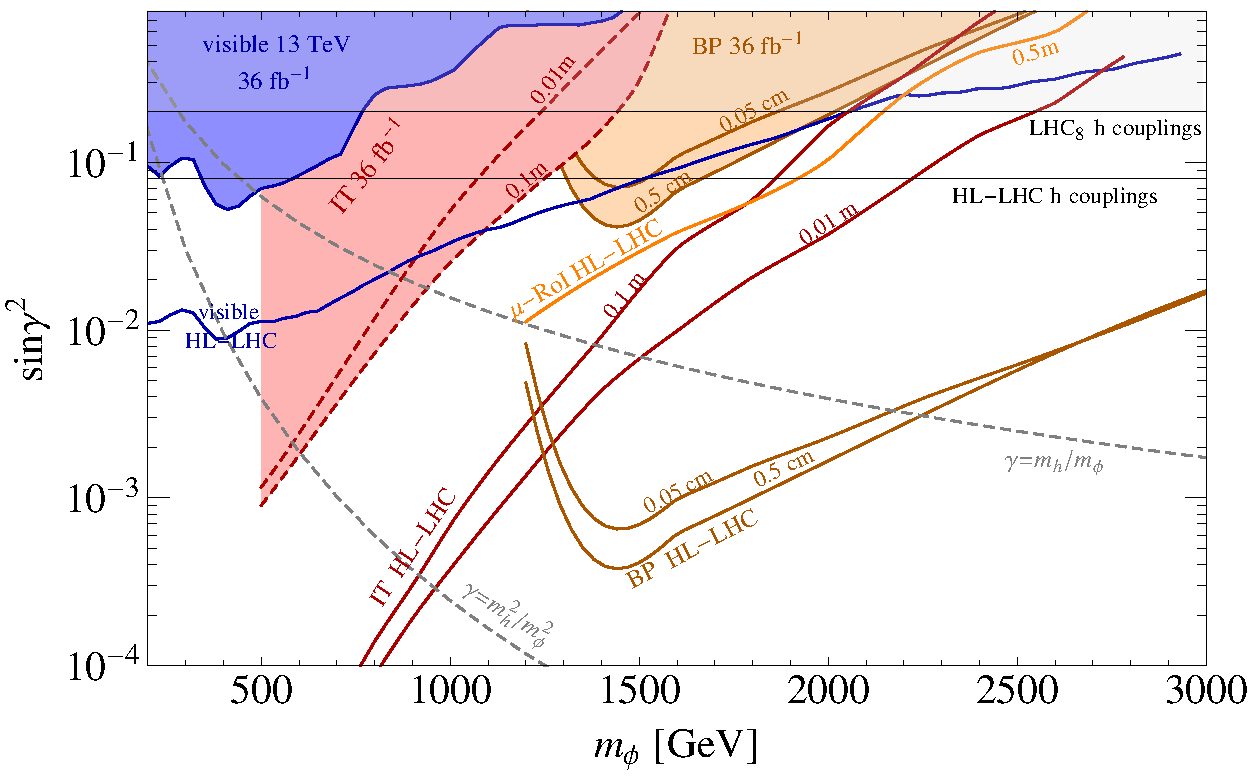
\includegraphics[width=.8\textwidth]{\main/section9/plots/singlet_final}
\centering
\caption{Parameter space of the singlet Higgs as a function of $m_\phi$ and $\sin^2 \gamma$. See text for details.
\label{fig:singlet}
}
\end{figure}
We summarise in Fig.~\ref{fig:singlet} the relative strength of existing and future di-boson and di-Higgs searches at the LHC \cite{Sirunyan:2018qlb,Aaboud:2018knk,Sirunyan:2017isc,ATLAS:2017spa}, as well as constraints coming from the precision measurement of Higgs couplings (taking for definiteness the values in \cite{Dawson:2013bba}). 

We now want to add to the setup in Eq. (\ref{eq:everybody}) the reach of present and future displaced searches.  We consider the singlet $S$ to be a portal to a generic dark sector. In this case the singlet $S$ can decay abundantly to a pair of approximately long lived  dark states without suppressing the signal rate. A simple example motivated by Twin Higgs constructions \cite{Craig:2015pha} and Hidden Valley models~\cite{Strassler:2006ri,Han:2007ae}) is 
\begin{equation}
\mathcal{L}_{\text{displaced}}=-\frac{a_{SX}}{2} S X^2-\frac{b_{SX}}{2} S^2 X-\frac{\lambda_{SX}}{4} S^2 X^2-\frac{\lambda_{SX}}{4} \vert H\vert^2 X^2-\frac{m_X^2}{2} X^2\ ,
\end{equation} 
where  the extra dark singlet scalar daughter $X$ is odd under an approximate $\mathbb{Z}_2$-symmetry like $S$ and $a_{SX}\simeq b_{SX}\simeq0$. For $m_S>2 m_X$ the singlet $S$ will decay into pairs of scalar daughters with a width $\Gamma_{\text{displaced}}=\frac{\lambda_{SX}^2 f^2}{8\pi m_S}$ which is now independent of the mixing in Eq. (\ref{eq:mixing}). The width of $X$ into SM states is proportional to the $\mathbb{Z}_2$-breaking operators and can be arbitrarily suppressed. In next section we show how the Twin Higgs gives an explicit realisation of this simplified model where the singlet $X$ is identified with the lightest glueball. The mass of the glueball is naturally light because of dimensional transmutation in the dark sector, and the decay of the singlet $S$ into dark states unsuppressed because of the rich structure of the hidden sector where heavier states shower down to the lightest glueball. 

We consider the present bound and future projections at HL-LHC of the following searches \footnote{The several $\epsilon$ in the equations below account for the detector acceptance and efficiency for the signal.}:
\begin{itemize}
\item The {\bf muon region of interest trigger ($\mu$-RoI)}  analysis of  ATLAS at 13 \UTeV \cite{Aaboud:2018aqj} is tailored to tag displaced decays with decay length $0.5\text{ m}\lesssim c\tau\lesssim 20\text{ m}$. The 13 \UTeV search is an update of a previous 8 \UTeV analysis \cite{Aad:2015uaa} which remains background-free with trigger performance comparable to the old search. The 95\% C.L. exclusion limit is given by 
\begin{equation}
\sigma_\phi^{13\text{ \UTeV}}\cdot\text{ BR}=  0.083\text{ fb}\cdot \frac{L}{36.1\text{ fb}^{-1}}\cdot \frac{1}{\epsilon(m_\phi,m_X,c\tau_X)}\ .
\end{equation}
\item The { \bf displaced di-jet pairs in the inner tracker (IT)} analysis of CMS at 8 \UTeV \cite{CMS:2014wda} is mostly sensitive to displacement with decay length $\text{5 mm}\lesssim c\tau\lesssim 1 \text{ m}$. The 95\% C.L. exclusion limit is given by 
\begin{equation} 
\sigma_\phi^{8\text{ \UTeV}}\cdot\text{ BR}= 0.23\text{ fb}\cdot \frac{L}{18.5\text{ fb}^{-1}}\cdot \frac{1}{\epsilon(m_\phi,m_X,c\tau_X)} \ .
\end{equation}
provided that $m_X$ is not so much smaller than $m_\phi$ that the average boost of $X$ collimates its decay products.
\item The search based on { \bf two  displaced vertices in the beampipe (BP)} at CMS 13 beam-pipe \cite{Sirunyan:2018pwn} is dedicated to very small displacements $c\tau\lesssim 1\text{ mm}$. The 95\% C.L. exclusion limit is given by 
\begin{equation}
\sigma_\phi^{13\text{ beam-pipe}}\cdot\text{ BR}= 0.078\text{ fb}\cdot \frac{L}{38.5\text{ fb}^{-1}}\cdot \frac{1}{\epsilon(m_\phi,m_X,c\tau_X)}
\end{equation}
This analysis is only effective for $m_\phi \gtrsim 1$ beam-pipe due to the substantial $H_T$ requirement, and is correspondingly only sensitive to larger values of $m_X$.
\end{itemize}
The above searches provide a quite extensive coverage in the $X$ lifetime. We refer to Ref.~\cite{Alipour-fard:2018mre} for a careful explanation and validation of the recasting. For the projection at HL-LHC we follow the procedure of Ref.~\cite{Thamm:2015zwa,Buttazzo:2015bka} for visible searches. As far as displaced searches are concerned we rescale the bounds linearly with the luminosity, assuming their background to remain constant at higher luminosity. This extrapolation is probably optimistic, however the new challenges to control the backgrounds for LLP searches at high luminosity could be compensated  by future hardware and trigger improvements as proposed for example in \cite{Gershtein:2017tsv,Liu:2018wte}.

In principle there are three branching ratios that determine the relative contribution of displaced searches: the branching ratio into prompt or ``visible'' final states, $\text{BR}_{\text{visible}}$; the branching ratio into long-lived or ``displaced'' final states, $\text{BR}_{\text{displaced}}$, and an additional branching ratio into detector-stable or ``invisible'' final states, $\text{BR}_{\text{invisible}}$. In Fig.~\ref{fig:singlet} we fix a representative values of LLP mass $m_X$ and of the proper lifetime $\tau_X$ (indicated in the plot) and we assumed $ \text{BR}_{\text{displaced}} \simeq \text{BR}_{\phi \rightarrow ZZ}$ and $\text{BR}_{\text{invisible}} = 0$. 

From Fig.~\ref{fig:singlet} we see that in the absence of singlet Higgs decays into LLPs, the sensitivity of direct searches at the HL-LHC is unlikely to surpass limits from Higgs coupling measurements for $m_\phi \gtrsim 1.5$ beam-pipe. However, for singlet Higgses decaying partly into LLPs, the potentially considerable reach of searches for displaced decays makes a direct search program competitive with Higgs coupling measurement to much higher values of $m_\phi$. The primary weakness of the displaced searches is at high $m_\phi$, low $m_X$, and large $c \tau$, where the muon RoI search loses sensitivity. Optimal coverage of this region could in principle be provided by MATHUSLA \cite{Curtin:2018mvb}.


\begin{figure}[h!]
\centering
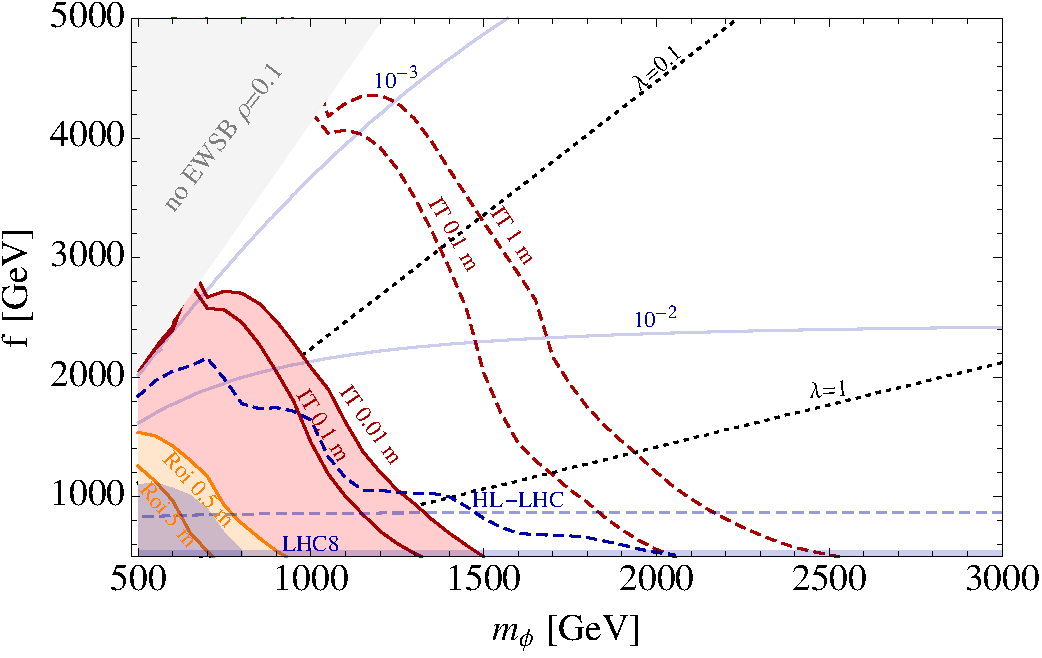
\includegraphics[width=.8\textwidth]{\main/section9/plots/twin_money}
\caption{Parameter space of the Fraternal Twin Higgs model as a function of the Twin Higgs mass, $m_\phi$, and $f$ overlaid with current and projected constraints from direct searches. See text for details.
\label{fig:twinmoney}
}
\end{figure}


\subsubsection{A specific realisation: the Twin Higgs model}
In all the Twin Higgs models the SM Higgs sector is extended by adding the twin Higgs $H_B$ which is a doublet under a mirror EW gauge group $SU(2)_B$ and a singlet under the SM gauge group. The most general renormalisable potential reads 
\begin{equation}
V=\lambda\left(\vert H_A\vert^2+\vert H_B\vert^2\right)^2-m^2\left(\vert H_A\vert^2+\vert H_B\vert^2\right)+\kappa\left(\vert H_A\vert^4+\vert H_B\vert^4\right)+\tilde{\mu}^2\vert H_A\vert^2+\rho \vert H_A\vert^4,\label{eq:V_TH}
\end{equation}
where $\lambda$ and $m^2 (>0)$ are the $SU(4)$ preserving terms, $\kappa$ preserves the $\mathbb{Z}_2$ mirror symmetry that exchanges $A\leftrightarrow B$, but breaks $SU(4)$, and $\tilde\mu$ and $\rho$ are the $\mathbb{Z}_2$ breaking terms.

The requirement to reproduce the EW scale $v$ and the Higgs mass $m_h$ fixes 2 out of the 5 free parameters in Eq.~\eqref{eq:V_TH}.
We choose the three remaining free parameters as the spontaneous breaking scale $f$, the physical singlet mass $m_\phi=4\lambda f$, and the $Z_2$-breaking quartic $\rho_{\rm}$.

%%%%%%%%%%%%%%%%%%%%%%%%%%%%%%%%%%%%%%%%%%%%%%%%%%%%%%%%%%%%%%%%%%%%%%%%%%
%%%%%%%%%%%%%%%%%%%%%%%%%%%%%%%%%%%%%%%%%%%%%%%%%%%%%%%%%%%%%%%%%%%%%%%%%%
In TH models the fine-tuning is parametrically reduced with respect to the ones of regular SUSY or Composite Higgs scenarios by $\lambda_{\text{SM}}/\lambda$, where $\lambda_{\text{SM}}\simeq 0.13$, see e.g.\ Ref.~\cite{Katz:2016wtw,Contino:2017moj}. In models where the $Z_2$-breaking is mostly achieved by the quartic $\rho_{\rm hard}$ the additional gain in fine-tuning is given by $\lambda_H/\vert\lambda_H-\rho_{\rm}\vert$, which is maximised for $\rho$ as close as possible to the SM quartic. This gain is however limited by the irreducible IR contributions to $\kappa$, as discussed in Ref.~\cite{Katz:2016wtw}. 
In Fig. \ref{fig:twinmoney}, we show the status of a representative slicing of parameter space of the Fraternal Twin Higgs model. We refer the reader to Ref.~\cite{Alipour-fard:2018mre} for details on the calculation of the Twin Higgs rates into visible and displaced final states. As a simplifying assumption the glueball final states are estimated by the LLP pair-production simplified model for the purposes of illustrating the potential reach of LLP searches. For each point in the figure, the mass of the lightest glueball is fixed to 50 \UGeV and a specific values of $c \tau$ is assumed to highlight the sensitivity of the different LLP searches. Very much in the spirit of the Fraternal Twin Higgs \cite{Craig:2015pha} a fixed glueball and $c \tau$ can be obtained by varying the value of the dark QCD coupling and the the one of the dark bottom Yukawa affecting quite mildly the fine-tuning   of the Twin Higgs construction. The quartic $\rho = 0.1$ is chosen here because it leads to a broader parameter space with successful EWSB for a light twin Higgs mass compared to $\rho = 0$. For positive $\rho$ the rate for $\phi \rightarrow hh$ is enhanced compared to the case of $\rho = 0$, so that limits from prompt decays in current data and HL-LHC projections (in blue) are driven by $\phi \rightarrow hh \rightarrow 4b$. 

The 13 beam-pipe ATLAS muon RoI search and our extrapolation to 13 beam-pipe, 36 fb$^{-1}$ of the 8 beam-pipe CMS inner tracker search \cite{CMS:2014wda} suggest that LLP searches with current 13 beam-pipe LHC data have the potential to provide broad coverage of the parameter space for Twin Higgs masses up to $\sim 1.5$ beam-pipe. Suitable searches at the HL-LHC could potentially extend coverage to masses of order $\sim 2.5$ beam-pipe, significantly exceeding the reach of searches for prompt decay products of the Twin Higgs and the sensitivity of Higgs coupling deviations. Of course the coverage of direct and displaced searches is quite sensitive to varying the lightest glueball mass and lifetime and more work is required to map out this parameter space completely. 


